\documentclass{icsc}

\usepackage{booktabs}  % nice tables
\usepackage{natbib}
\usepackage{siunitx}  % use for all units
\usepackage{subcaption}  % for subfigures

\def\kph{\kilo\meter\per\hour}

\pagestyle{empty}

\begin{document}

\begin{center}
  \fontsize{14}{20}{\bf Balance Assist Bicycle Reduces Undesired Motions and
    Fall Probability when Subject to Disturbances\\[3pt]}
\end{center}

%%%%%%%%%%%%%%%% authors %%%%%%%%%%%%%%%
\begin{center}
  \normalsize{\bf{J. K. Moore,
                  M. Haitjema,
                  L. Alizadehsaravi}}
\end{center}

\begin{center}
  \begin{tabular}{c}
    Faculty of Mechanical Engineering\\
    Delft University of Technology\\
    Mekelweg, 2628CD Delft, The Netherlands\\
    e-mail: j.k.moore@tudelft.nl\\
  \end{tabular}
\end{center}

\begin{keywords}
  bicycle,
  fall,
  assist,
  control,
  perturbation
\end{keywords}

\section{INTRODUCTION}
%
We have developed a balance assisting bicycle that uses a custom electric motor
to apply a steering torque in parallel with the rider's steering actions. The
motor is controlled by a simple control algorithm based on feedback from a rate
gyroscope that measures vehicle roll angular rate. Applying a steering torque
in the same direction and proportional to the rolling rate can lower the speed
range at which the bicycle feels self-stable to the rider. We hypothesize that
making the bicycle stable at lower speeds will reduce the control action needed
from the rider in basic balancing tasks and that use of such a system may
reduce falls. We have developed three comprehensive experiments to assess the
effectiveness of the balance assist effects. In the first experiments, we both
distract the rider and apply small disturbances via the steering motor during
straight line balancing. In the second experiment, we apply increasingly large
perturbations to the handlebars via computer controlled ropes while riding on a
treadmill at low speeds. In the final experiment, we perturb straight line
riding via a kickplate, which slides the ground out from under the front wheel
of the bicycle to see differences in recovery response with and without balance
assist enabled.

\section{METHODS}
%
To design the controller, we utilized the linear Carvallo-Whipple bicycle model
from \cite{Meijaard2007}. The states are the roll angle \(\phi\) and steer
angle \(\delta\) along with their time derivatives and the inputs are roll
torque \(T_\phi\) and steer torque \(T_\delta\). The state \(\mathbf{A}\) and
input \(\mathbf{B} = \begin{bmatrix}\mathbf{B}_\phi \quad
\mathbf{B}_\delta\end{bmatrix} \) matrices are functions of the equilibrium
forward speed \(v\). The applied steering torque \(T_\delta\) is the sum of the
(h)uman and (m)otor torques, with the motor torque following a proportional
roll rate feedback law scheduled by speed, similar to that shown in
\cite{Schwab2008}:
%
\begin{align}
  T_\delta =
  T_\delta^\textrm{h} + T_\delta^\textrm{m} =
  T_\delta^\textrm{h} - k_{\dot{\phi}}(v - v_\textrm{weave})\dot{\phi}
\end{align}
where \(v_\textrm{weave}\) is the bicycle's open loop weave critical speed.
This gives the closed loop model with the automatic control:
%
\begin{align}
  \dot{\vec{x}} =
  \left(
    \mathbf{A} - \mathbf{B}_\delta
    \left[0 \quad k_{\dot{\phi}}(v - v_\textrm{weave}) \quad 0 \quad 0\right]
  \right)
  \begin{bmatrix} \phi \\ \dot{\phi} \\ \delta \\ \dot{\delta} \end{bmatrix} +
  \mathbf{B}
  \begin{bmatrix} T_{\phi} \\ T_\delta^\textrm{h} \end{bmatrix}
  \label{eq:state-space}
\end{align}

The gain \(k_{\dot{\phi}}\) can be selected such that the eigenvalues of
Equation~\ref{eq:state-space} have negative real parts for a range of speeds,
making the bicycle stable.

We developed a series of three experiments to assess whether stabilizing the
bicycle is beneficial in safety critical scenarios:
\begin{description}
  \item[Experiment 1] Comparison of 18 older and 14 younger adults in straight
    line riding when 1) looking over their shoulder and 2) subjected steer
    motor induced perturbations with the assist on and off. We measured the
    standard deviation of their steer and roll motions after the disturbances.
  \item[Experiment 2] Twenty-six young adults were subjected to externally
    applied and measured handlebar torques of varying magnitudes while riding
    on a treadmill at low speeds 6~\si{\kph} and 10~\si{\kph} to determine the
    magnitude of perturbation required to cause them to fall with the balance
    assist system on and off. We log the order of perturbations and their
    impulse as well as the bicycle state at the time of perturbation.
  \item[Experiment 3] We subject 11 participants riding at 12~\si{\kph} to
    lateral pulse-like perturbations at the front tire contact patch as they
    rode over a kickplate. We measured the standard deviation of their steer
    and roll motions after the disturbances.
\end{description}

\begin{figure}
  \begin{center}
    \subcaptionbox{Experiment 1: Course layout (left) and GNSS traces
    (right).}{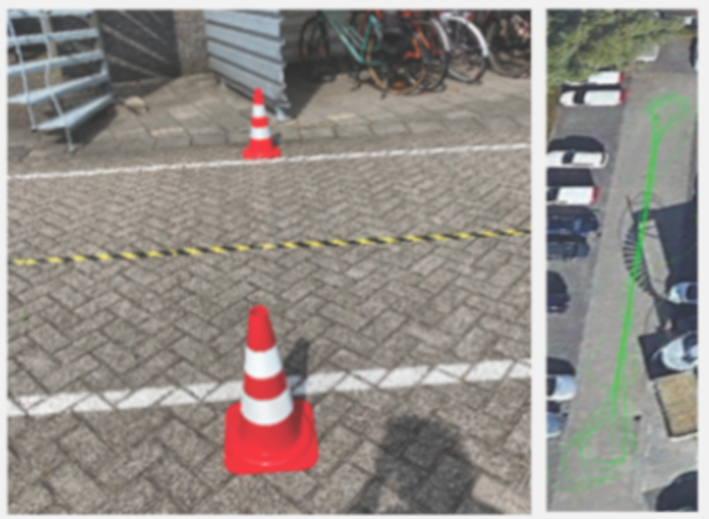
\includegraphics[width=50mm]{old-young-disturbance-experiments.png}}
    \subcaptionbox{Experiment 2: During (left) and after (right) handlebar
    perturbation.}{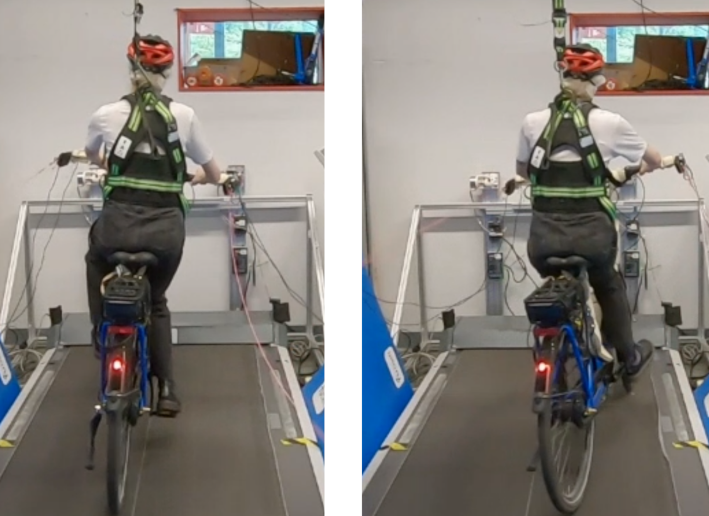
\includegraphics[width=50mm]{perturbation-threshold-experiment.png}}
    \subcaptionbox{Experiment 3: Just after leftward front wheel
    kick.}{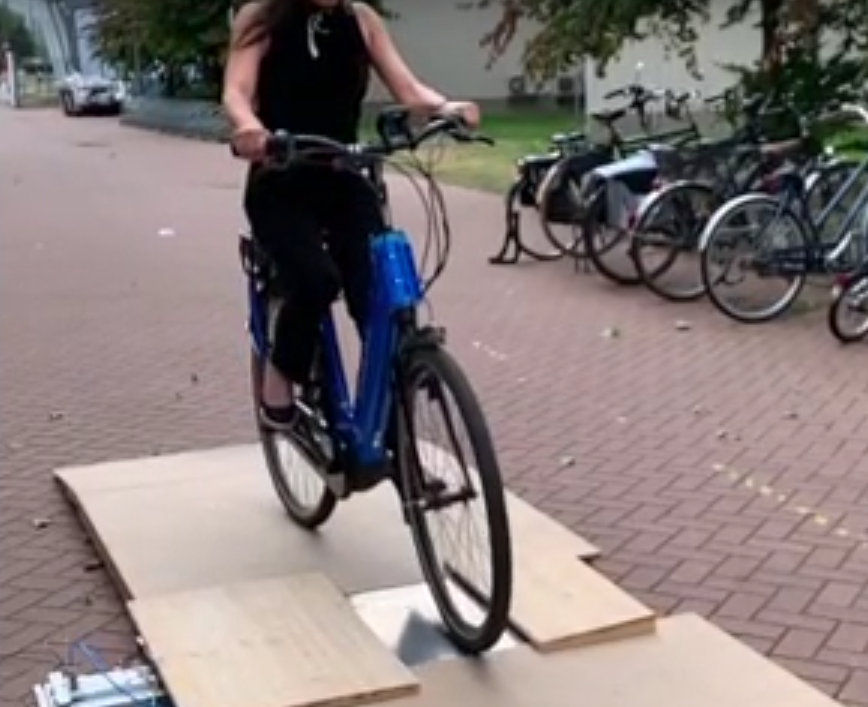
\includegraphics[width=45mm]{kickplate-experiment.png}}
    \caption{Representative images from each experiment.}
    \label{fig:experiments}
  \end{center}
\end{figure}

For analysis, we apply multivariate linear regression to the performance
metrics derived from each experiment (ANOVA in Experiments 1 \& 3, logistic in
Experiment 2) and investigate whether the balance assist system reduce response
motions (Experiments 1 \& 3) or the probability of falling is reduced
(Experiment 2).

\section{Results}
%
In Experiment 1, we found that the standard deviation of the roll rate during
straight riding is reduced when the balance assist system is turned on for both
young and old participants. In Experiment 2, the probability of falling is
significantly reduced while riding at 6~\si{\kph} when the balance assist
system is on. There is also a reduction in probability at 10~\si{\kph}, but
the effect was not statistically significant (\(P=0.7\)). In Experiment 3, we
found that the standard deviation of steer angle, roll angle, and yaw angle are
all significantly reduced post perturbation when the balance assist system is
on.

\begin{figure}[t]
  \begin{center}
    \subcaptionbox{Results 1: Roll rate
    reduction.}{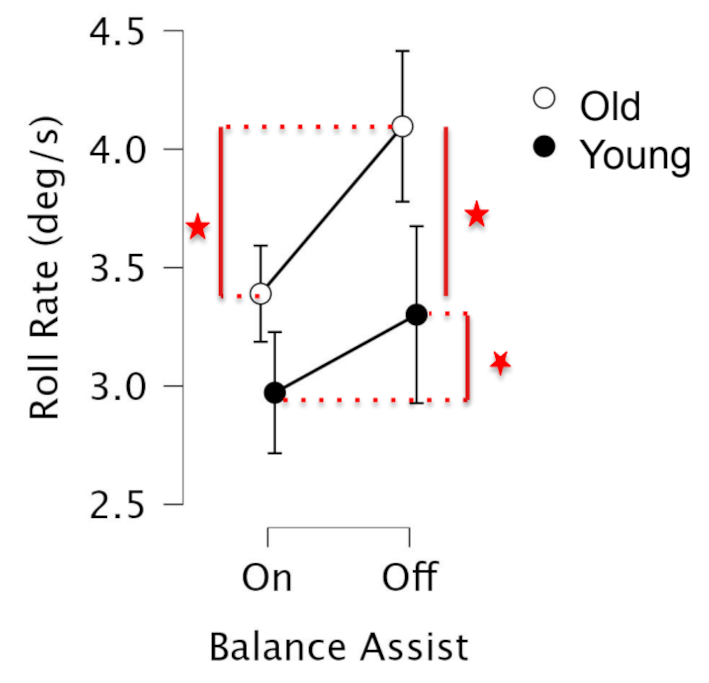
\includegraphics[width=60mm]{old-young-disturbance-results.png}}
    \subcaptionbox{Results 2: Fall probability as a function of perturbation
    impulse.}{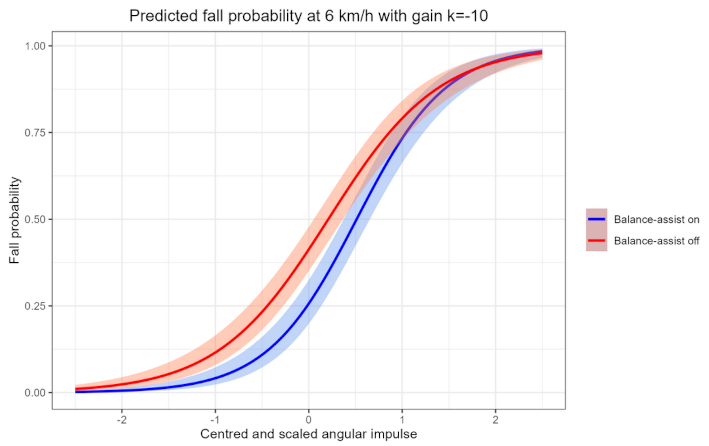
\includegraphics[width=80mm]{perturbation-threshold-results.png}}
    \subcaptionbox{Results 3: Yaw angle
    reduction.}{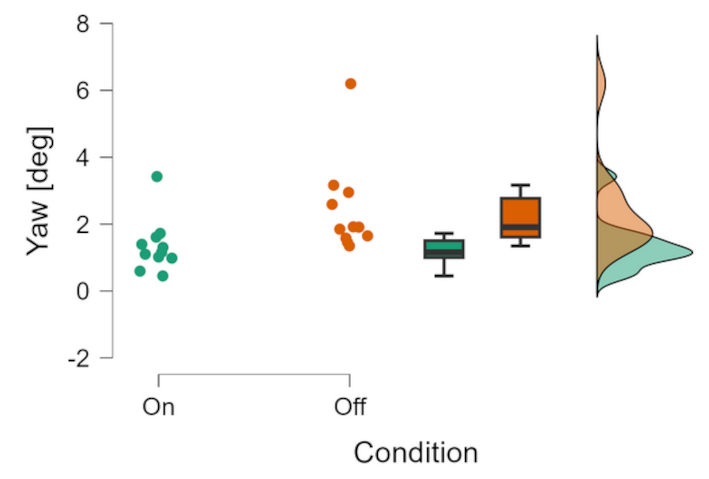
\includegraphics[width=60mm]{kickplate-results.png}}
    \caption{Representative results from each experiment.}
    \label{fig:fig2}
  \end{center}
\end{figure}

\section{CONCLUSIONS}
%
The balance assist system, consisting of roll rate feedback steering control,
stabilizes the riderless bicycle at speeds greater than approximately
4~\si{\kph} which is much lower than the uncontrolled stable speeds of greater
than 18~\si{\kph}. The bicycle is rideable and we show that motions resulting
from disturbances and distractions are reduced with the system is on. We also
show that the probability of falling is significantly reduced at low speeds
when the system is on. Given that large steer and roll motions correlate to
reduced rider control authority and that many single actor falls occur at low
speeds~\cite{Wegman2024}, we project that wide use of a balance assisted
bicycle may reduce falls and thus injuries.

\bibliographystyle{plain}
\bibliography{references}

\end{document}
